\documentclass[11pt,a4paper]{article}

% définition des marges du document
\setlength{\topmargin}{0cm}
\setlength{\headheight}{0.4cm}
\setlength{\headsep}{0.8cm}
\setlength{\footskip}{1cm}
\setlength{\textwidth}{17cm}
\setlength{\textheight}{25cm}
\setlength{\voffset}{-1.5cm}
\setlength{\hoffset}{-0.5cm}
\setlength{\oddsidemargin}{0cm}
\setlength{\evensidemargin}{0cm}

\usepackage[
        backend=biber,
        style=phys,  
        mcite=true,
        subentry,
        hyperref=true,
        ]{biblatex}
\addbibresource{Rapport.bib}

\usepackage{graphicx} % inclusion des figures
\usepackage{tabularx} % gestion avancée des tableaux

\usepackage{physics}
\usepackage{amsmath} % collection de symboles mathématiques
\usepackage{amssymb} % collection de symboles mathématiques

\usepackage[utf8]{inputenc}
\usepackage[T1]{fontenc}
\DeclareUnicodeCharacter{2212}{-}

\usepackage[english]{babel}

\usepackage{siunitx}
\usepackage[version=4]{mhchem}


\usepackage{xcolor} % gestion de différentes couleurs

\definecolor{linkcolor}{rgb}{0,0,0.6} % définition de la couleur des liens pdf
\usepackage[ pdftex,colorlinks=true,
pdfstartview=FitV,
linkcolor= linkcolor,
citecolor= linkcolor,
urlcolor= linkcolor,
hyperindex=true,
hyperfigures=false]
{hyperref} % fichiers pdf 'intelligents', avec des liens entre les références, etc.
\usepackage{fancyhdr} % entêtes et pieds de pages personnalisés

% définition de l'entête et du pied de page
\pagestyle{fancy}
\fancyhead[L]{\scriptsize \textsc{Perturbation theory in the complex plane}}
\fancyhead[R]{\scriptsize \textsc{Antoine \textsc{MARIE}}}
\fancyfoot[C]{ \thepage}

\newcommand{\bH}{\mathbf{H}}
\newcommand{\bV}{\mathbf{V}}

\begin{document}

% Pour faciliter la mise en forme de la page du titre, on supprime l'indentation automatique en début de paragraphe
\setlength{\parindent}{0pt}

% Pas d'en-tête ni de pied pour la première page
\thispagestyle{empty}


\includegraphics[height=2cm]{logoens.eps} \hfill 
\includegraphics[height=2cm]{logoucbl.eps} \hfill 
\includegraphics[height=2cm]{logounivlyon.eps}
\vspace{0.5cm}

\begin{tabularx}{\textwidth}{@{} l X l @{} }
{\sc Licence / Master Science de la matière} & & Stage 2019-2020 \\
{\it École Normale Supérieure de Lyon} & & Antoine \textsc{MARIE} \\
{\it Université Claude Bernard Lyon I} & & M1 Chimie
\end{tabularx}

\begin{center}

\vspace{1.5cm}

\rule[11pt]{5cm}{0.5pt}

\textbf{\huge Pertubation theories in the complex plane}

\rule{5cm}{0.5pt}

\vspace{1.5cm}

\parbox{15cm}{\small
\textbf{Abstract} : \it In this work, we explore the description of quantum chemistry in the complex plane. We see that the physics of the system can be connected to the position of the energy singularities in the complex plane. After a brief presentation of the fundamental notions of quantum chemistry and perturbation theory in the complex plane, we perform an historical review of the researches that have been done on the physic of singularities. Then we connect all those points of view on this problem using the spherium model (i.e., two opposite-spin electrons restricted to remain on the surface of a sphere of radius $R$) as a theoretical playground. In particular, we explore the effects of symmetry breaking of the wave functions on the singularity structure.
}

\vspace{0.5cm}

\parbox{15cm}{
\textbf{Keywords} : \it Quantum chemistry, Perturbation theory,  Spherium, Exceptional points, Symmetry breaking
} %fin de la commande \parbox des mots clefs

\vspace{0.5cm}

\parbox{15cm}{
Internship supervisor:

{\bf Pierre-François \textsc{LOOS}}

\href{mailto:loos@irsamc.ups-tlse.fr}{\tt loos@irsamc.ups-tlse.fr} / tél. (+33) 5 61 55 73 39

Laboratoire de Chimie et Physique Quantiques

{\it 118, route de Narbonne

31062 Toulouse - France}

\url{https://www.irsamc.ups-tlse.fr/}
} %fin de la commande \parbox encadrant / laboratoire d'accueil

\vspace{0.5cm}

\includegraphics[height=2cm]{LCPQ_logo.pdf} \hfill 
\includegraphics[height=2cm]{LogoCNRS.eps} \hfill 
\includegraphics[height=2cm]{UPS_logo.jpg}

\end{center}

\vfill
\hfill \today

\newpage

\setlength{\parindent}{17pt}

\section*{Acknowledgments}

\tableofcontents

\newpage

%============================================================%
\section{Introduction}
%============================================================%

It has always been of great importance for theoretical chemists to better understand excited states and their properties because processes involving excited states are ubiquitous in nature (physics, chemistry and biology). One of the major challenges is to accurately compute energies of a chemical system (atoms, molecules, ..). Plenty of methods have been developed to this end and each of them have its own advantages but also its own flaws. The fact that none of all those methods is successful for every molecule in every geometry encourages chemists to continue the development of new methodologies to get accurate energies and to try to deeply understand why each method fails or not in each situation. All those methods rely on the notion of quantised energy levels of Hermitian quantum mechanics. In quantum chemistry, the ordering of the energy levels represents the different electronic states of a molecule, the lowest being the ground state while the higher ones are the so-called excited states. We need methods to accurately get how those states are ordered.

Within this quantised paradigm, electronic states look completely disconnected from one another.
However, one can gain a different perspective on quantisation extending quantum chemistry into the complex domain.
In a non-Hermitian complex picture, the energy levels are \textit{sheets} of a more complicated topological manifold called \textit{Riemann surface}, and they are smooth and continuous \textit{analytic continuation} of one another.
In other words, our view of the quantised nature of conventional Hermitian quantum mechanics arises only from our limited perception of the more complex and profound structure of its non-Hermitian variant.

Therefore, by analytically continuing the energy $E(\lambda)$ in the complex domain (where $\lambda$ is a coupling parameter), the ground and excited states of a molecule can be smoothly connected.
This connection is possible because by extending real numbers to the complex domain, the ordering property of real numbers is lost.
Hence, electronic states can be interchanged away from the real axis since the concept of ground and excited states has been lost.
Amazingly, this smooth and continuous transition from one state to another has recently been experimentally realized in physical settings such as electronics, microwaves, mechanics, acoustics, atomic systems and optics. \cite{Bittner_2012, Chong_2011, Chtchelkatchev_2012, Doppler_2016, Guo_2009, Hang_2013, Liertzer_2012, Longhi_2010, Peng_2014, Peng_2014a, Regensburger_2012, Ruter_2010, Schindler_2011, Szameit_2011, Zhao_2010, Zheng_2013, Choi_2018, El-Ganainy_2018}


Exceptional points (EPs) \cite{Heiss_1990, Heiss_1999, Heiss_2012, Heiss_2016} are non-Hermitian analogs of conical intersections (CIs) \cite{Yarkony_1996} where two states become exactly degenerate.
CIs are ubiquitous in non-adiabatic processes and play a key role in photo-chemical mechanisms.
In the case of auto-ionizing resonances, EPs have a role in deactivation processes similar to CIs in the decay of bound excited states.
Although Hermitian and non-Hermitian Hamiltonians are closely related, the behavior of their eigenvalues near degeneracies is starkly different.
For example, encircling non-Hermitian degeneracies at EPs leads to an interconversion of states, and two loops around the EP are necessary to recover the initial energy (see \autoref{fig:TopologyEP} for a graphical example).
Additionally, the wave function picks up a geometric phase (also known as Berry phase \cite{Berry_1984}) and four loops are required to recover the initial wave function.
In contrast, encircling Hermitian degeneracies at CIs only introduces a geometric phase while leaving the states unchanged.
More dramatically, whilst eigenvectors remain orthogonal at CIs, at non-Hermitian EPs the eigenvectors themselves become equivalent, resulting in a \textit{self-orthogonal} state. \cite{MoiseyevBook}
More importantly here, although EPs usually lie off the real axis, these singular points are intimately related to the convergence properties of perturbative methods and avoided crossing on the real axis are indicative of singularities in the complex plane. \cite{Olsen_1996, Olsen_2000} 

\begin{figure}[h!]
    \centering
    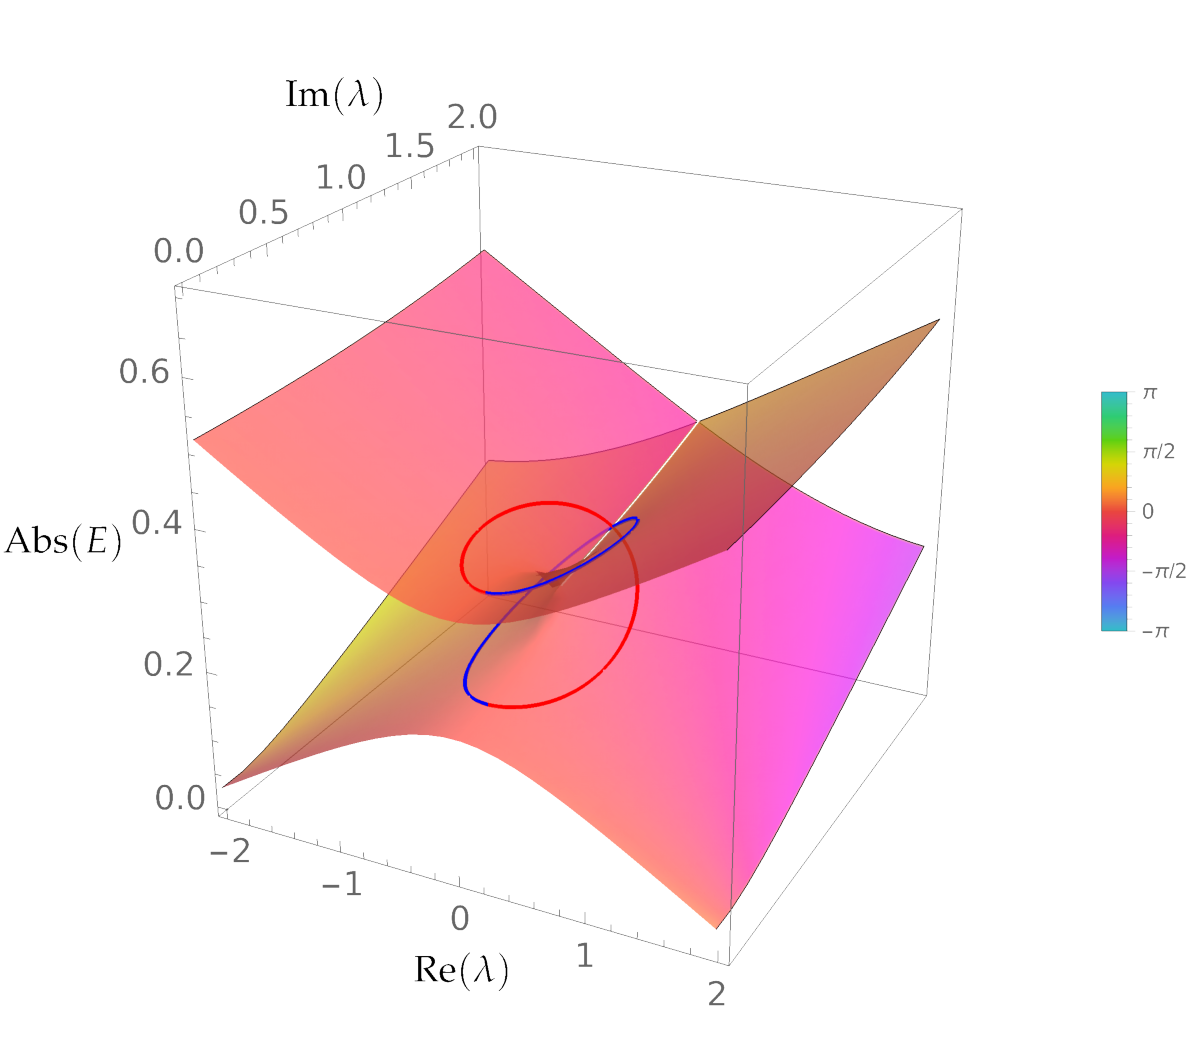
\includegraphics[width=0.7\textwidth]{TopologyEP.pdf}
    \caption{\centering A generic EP with the square root branch point topology. A loop around the EP interconvert the states.}
    \label{fig:TopologyEP}
\end{figure}

%============================================================%
\section{Perturbation theory}
%============================================================%

Within (time-independent) Rayleigh-Schr\"odinger perturbation theory, the Schr\"odinger equation 
\begin{equation} \label{eq:SchrEq}
	\bH \Psi = E \Psi
\end{equation} 
is recast as 
\begin{equation} \label{eq:SchrEq-PT}
	\bH(\lambda) \Psi(\lambda) = (\bH^{(0)} + \lambda \bV ) \Psi(\lambda) = E(\lambda) \Psi(\lambda),
\end{equation}
where $\bH^{(0)}$ is the zeroth-order Hamiltonian and $\bV = \bH - \bH^{(0)}$ is the so-called perturbation.
The ``physical'' system of interest is recovered by setting the coupling parameter $\lambda$ to unity.
This decomposition is obviously non-unique and motivated by several factors as discussed below.

Accordingly to Eq.~\eqref{eq:SchrEq-PT}, the energy can then be written as a power series of $\lambda$
\begin{equation} \label{eq:Elambda}
	E(\lambda) = \sum_{k=0}^\infty \lambda^k E^{(k)}
\end{equation}
However it is not guaranteed that the series \eqref{eq:Elambda} has a radius of convergence $\abs{\lambda_0} < 1$. 
In other words, the series might well be divergent for the physical system at $\lambda = 1$. 
One can prove that the actual value of the radius of convergence $\abs{\lambda_0}$ can be obtained by looking for the singularities of $E(\lambda)$ in the complex $\lambda$ plane.
This is due to the following theorem \cite{Goodson_2012}: 
\begin{quote}
	\textit{``The Taylor series about a point $z_0$ of a function over the complex $z$ plane will converge at a value $z_1$ if the function is non-singular at all values of $z$ in the circular region centered at $z_0$ with radius $\abs{z_1 − z_0}$. If the function has a singular point $z_s$ such that $\abs{z_s − z_0} < \abs{z_1 − z_0}$, then the series will diverge when evaluated at $z_1$.''}
\end{quote}
This theorem means that the radius of convergence of the perturbation series is equal to the distance to the origin of the closest singularity of $E(\lambda)$.  

The discovery of a partitioning of the Hamiltonian that allowed chemists to recover a part of the correlation energy (i.e. the difference between the exact energy and the Hartree-Fock energy) using perturbation theory has been a major step in the development of post-Hartree-Fock methods. This case of the Rayleigh-Schrödinger perturbation theory is called the M{\o}ller-Plesset perturbation theory \cite{Moller_1934}. In the MPPT the unperturbed Hamiltonian is the sum of the $n$ mono-electronic Fock operators which are the sum of the one-electron core Hamiltonian $h(i)$, the Coulomb $J_j(i)$ and Exchange $K_j(i)$ operators.
 
\begin{equation}
H_0= \sum\limits_{i=1}^{n} f(i)
\end{equation}

\begin{equation}
f(i) = h(i) + \sum\limits_{j=1,j \neq i}^{n} \left[J_j(i) - K_j(i)\right]
\end{equation}

In Hartree-Fock theory the exact wave function is approximated as a Slater-determinant (which is an anti-symmetric combination of mono-electronic orbitals) and those wave functions are eigenvectors of the Fock operators. In the perturbation theory the energy is a power series of $\lambda$ and the physical energy is obtained by taking $\lambda$ equal to 1. We will refer to the energy up to the $n$-th order as the MP$n$ energy. The MP0 energy overestimates the energy by double counting the electron-electron interaction, the MP1 corrects this effect and the MP1 energy is equal to the Hartree-Fock energy. The MP2 energy starts to recover a part of the correlation energy.

\begin{equation}
E_{\text{MP$_{n}$}}= \sum_{k=0}^n E^{(k)}
\end{equation}

But as mentioned before \textit{a priori} there are no reasons that this power series is always convergent for $\lambda$=1 when $n$ goes to infinity. In fact, it is known that when the Hartree-Fock wave function is a bad approximation of the exact wave function, for example for multi-reference states, the M{\o}ller-Plesset will give bad results\cite{Gill_1986, Gill_1988, Handy_1985, Lepetit_1988}. A smart way to investigate the convergence properties of the MP series is to transform the coupling parameter $\lambda$ into a complex variable. By doing so the Hamiltonian and the energy become functions of this variable. The energy becomes a multivalued function on $n$ Riemann sheets. As mentioned above by searching the singularities of the function $E(\lambda)$ we can get information on the convergence properties of the MPPT. Those singularities of the energy are exactly the exceptional points connecting the electronic states mentioned in the introduction. The direct computation of the terms of the series is quite easy up to the 4th order and the 5th and 6th order can be obtained at high cost. But to deeply understand the behavior of the MP series and how it is connected to the singularities, we need to have access to high order terms of the series. For small systems we can have access to the whole series using Full Configuration Interaction. If the Hamiltonian $H(\lambda)$ is diagonalized in the FCI basis set we get the exact energies (in this finite basis set) and expanding in $\lambda$ allows to to get the M{\o}ller-Plesset perturbation series at every order.

%============================================================%
\section{Historical overview}
%============================================================%

\subsection{Behavior of the M{\o}ller-Plesset series}

When we use M{\o}ller-Plesset perturbation theory it would be very convenient that each time a higher order term is computed the result obtained is closer to exact energy. In other words, that the M{\o]ller-Plesset series would be monotonically convergent. Assuming this, the only limiting process to get the exact correlation energy in a finite basis set is our ability to compute the terms of the perturbation series.
Unfortunately this is not true in generic cases and rapidly some strange behaviors of the series were exhibited. In the late 80's Gill et al. reported deceptive and slow convergences in stretch systems\cite{Gill_1986, Gill_1988, Handy_1985, Lepetit_1988}. In the \autoref{fig:RUMP_Gill} we can see that the restricted M{\o}ller-Plesset series is convergent but oscillating which is not convenient if you are only able to compute few terms (for example here RMP5 is worse than RMP4). On the other hand, the unrestricted M{\o}ller-Plesset series is monotonically converging (except for the first few orders) but very slowly so we can't use it for systems where we can only compute the first terms.

\begin{figure}[h!]
    \centering
    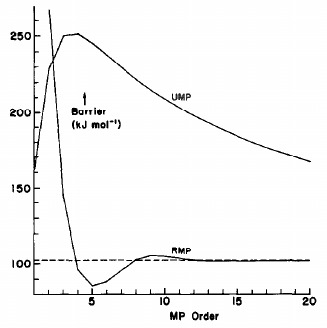
\includegraphics[width=0.45\textwidth]{gill1986.png}
    \caption{\centering Barriers to homolytic fission of \ce{He2^2+} at MPn/STO-3G level ($n = 1$--$20$)\cite{Gill_1986}.}
    \label{fig:RUMP_Gill}
\end{figure}

When a bond is stretched the exact function can undergo a symmetry breaking becoming multi-reference during this process (see for example the case of \ce{H_2} in \cite{SzaboBook}). A restricted HF Slater determinant is a poor approximation of a symmetry-broken wave function but even in the unrestricted formalism, where the spatial orbitals of electrons $\alpha$ and $\beta$ are not restricted to be the same\cite{Fukutome_1981}, which allows a better description of symmetry-broken system, the series doesn't give accurate results at low orders. Even with this improvement of the zeroth order wave function the series doesn't have the smooth and rapidly converging behavior wanted. 

\begin{table}[h!]
    \centering
    \begin{tabular}{c c c c c c c}
\hline
 $r$ & UHF & UMP2 & UMP3 & UMP4 & $\expval{S^2}$ \\
\hline
0.75 & 0.0\% & 63.8\% & 87.4\% & 95.9\% & 0.00\\
1.35 & 0.0\% & 15.2\% & 26.1\% & 34.9\% & 0.49\\
2.00 & 0.0\% & 01.0\% & 01.8\% & 02.6\% & 0.95\\
2.50 & 0.0\% & 00.1\% & 00.3\% & 00.4\% & 0.99\\
\hline
\end{tabular}
    \caption{\centering Percentage of electron correlation energy recovered and $\expval{S^2}$ for the \ce{H2} molecule as a function of bond length (r,\si{\angstrom}) in the STO-3G basis set \cite{Gill_1988}.}
    \label{tab:SpinContamination}
\end{table}

In the unrestricted framework the ground state singlet wave function is allowed to mix with triplet states which leads to spin contamination. Gill et al. highlighted the link between the slow convergence of the unrestricted MP series and the spin contamination of the wave function as shown in the \autoref{tab:SpinContamination} in the example of \ce{H_2} in a minimal basis. Handy and co-workers exhibited the same behaviors of the series (oscillating and monotonically slowly) in stretched \ce{H_2O} and \ce{NH_2} systems \cite{Handy_1985}. Lepetit et al. analyzed the difference between the M{\o}ller-Plesset and Epstein-Nesbet partitioning for the unrestricted Hartree-Fock reference \cite{Lepetit_1988}. They concluded that the slow convergence is due to the coupling of the single with the double excited configuration. Moreover the MP denominators tends towards a constant so each contribution become very small when the bond is stretched.

Cremer and He analyzed 29 FCI systems \cite{Cremer_1996} and regrouped all the systems in two classes. The class A systems which have a monotonic convergence to the FCI value and the class B which converge erratically after initial oscillations. The sample of systems contains stretched molecules and also some at equilibrium geometry, there are also some systems in various basis sets. They highlighted that systems with class A convergence have well-separated electrons pairs whereas class B systems present electrons clustering. This classification was encouraging in order to develop methods based on perturbation theory as it rationalizes the two different observed convergence modes. If it is possible to predict if a system is class A or B, then one can use extrapolation method of the first terms adapted to the class of the systems \cite{Cremer_1996}.

\subsection{Cases of divergence}

However Olsen et al. have discovered an even more preoccupying behavior of the MP series in the late 90's. They have shown that the series could be divergent even in systems that they considered as well understood like \ce{Ne} and \ce{HF} \cite{Olsen_1996, Christiansen_1996}. Cremer and He had already studied those two systems and classified them as class B systems. But Olsen and his co-workers have done the analysis in larger basis sets containing diffuse functions and in those basis sets the series become divergent at high order.

\begin{figure}[h!]
    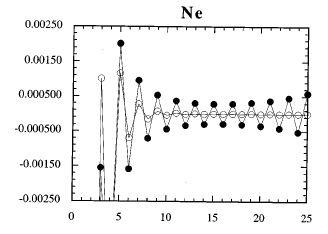
\includegraphics[height=5.5cm]{Nedivergence.png}
    \hfill
    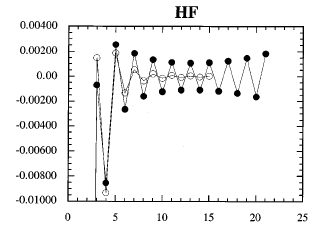
\includegraphics[height=5.5cm]{HFdivergence.png}
    \hfill
    \caption{\centering Correlation contributions for \ce{Ne} and \ce{HF} in the cc-pVTZ-(f/d) $\circ$ and aug-cc-pVDZ $\bullet$ basis sets.}
    \label{fig:my_label}
\end{figure}

The discovery of this divergent behavior was really worrying because in order to get more and more accurate results theoretical chemists need to work in large basis sets. As a consequence they investigated the causes of those divergences and in the same time the reasons of the different types of convergence. To do this they analyzed the relation between the dominant singularity (i.e. the closest singularity to the origin) and the convergence behavior of the series \cite{Olsen_2000}. Their analysis is based on Darboux's theorem: in the limit of large order, the series coefficients become equivalent to the Taylor series coefficients of the singularity closest to the origin. Following the result of this theorem, the convergence patterns of the MP series can be explained by looking at the dominant singularity.

A singularity in the unit circle is designated as an intruder state, more precisely as a front-door (respectively back-door) intruder state if the real part of the singularity is positive (respectively negative). The method used is to do a scan of the real axis to identify the avoided crossing responsible for the pair of dominant singularity. Then by modeling this avoided crossing by a two-state Hamiltonian one can get an approximation of the dominant conjugate pair of singularity by finding the EPs of the $2\times2$ Hamiltonian. The diagonal matrix is the unperturbed Hamiltonian and the other matrix is the perturbative part of the Hamiltonian.

\begin{equation}
\mqty(\alpha & \delta \\ \delta & \beta) = \mqty(\alpha + \alpha_s & 0 \\ 0 & \beta + \beta_s ) + \mqty(- \alpha_s & \delta \\ \delta & - \beta_s)
\end{equation}
 
They first studied molecules with low-lying doubly excited states of the same spatial and spin symmetry because in those systems the HF wave function is a bad approximation. The exact wave function has a non-negligible contribution from the doubly excited states, so those low-lying excited states were good candidates for being intruder states. For \ce{CH_2} in a large basis set, the series is convergent up to the 50th order. They showed that the dominant singularity lies outside the unit circle but close to it causing the slow convergence.

Then they demonstrated that the divergence for the \ce{Ne} is due to a back-door intruder state. When the basis set is augmented with diffuse functions, the ground state undergo sharp avoided crossings with highly diffuse excited states leading to a back door intruder state. They used their two-state model on this avoided crossings and the model was actually predicting the divergence of the series. They concluded that the divergence of the series was due to the interaction with a highly diffuse excited state. 

Moreover they proved that the extrapolation formula of Cremer and He \cite{Cremer_1996} can't be used for all systems. Even more, that those formula were not mathematically motivated when looking at the singularity causing the divergence. For example the hydrogen fluoride molecule contains both back-door intruder states and low-lying doubly excited states which results in alternated terms up to order ten and then the series is monotonically convergent. This is due to the fact that two pairs of singularity are approximately at the same distance from the origin.

\subsection{The singularity structure}

In the 2000's Sergeev and Goodson \cite{Sergeev_2005, Sergeev_2006}  analyzed this problem from a more mathematical point of view by looking at the whole singularity structure where Olsen and his co-workers were trying to find the dominant singularity causing the divergence. They regrouped singularities in two classes: the $\alpha$ singularities which have unit order imaginary parts and the $\beta$ singularities which have very small imaginary parts. The singularities $\alpha$ are related to large avoided crossing between the ground state and a low-lying excited states. Whereas the singularities $\beta$ come from a sharp avoided crossing between the ground state and a highly diffuse state. They succeeded to explain the divergence of the series caused by $\beta$ singularities using a previous work of Stillinger \cite{Stillinger_2000}. 

The M{\o}ller-Plesset Hamiltonian is defined as below and by reassembling the term we get the expression \eqref{eq:HamiltonianStillinger}.

\begin{equation}
H(\lambda)=H_0 + \lambda (H_\text{phys} - H_0)    
\end{equation}

\begin{equation}
    H_\text{phys}=\sum\limits_{j=1}^{n}\left[ -\frac{1}{2}\grad_j^2 - \sum\limits_{k=1}^{N} \frac{Z_k}{|\vb{r}_j-\vb{R}_k|}+\sum\limits_{j<l}^{n}\frac{1}{|\vb{r}_j-\vb{r}_l|}\right]
\end{equation}

\begin{equation}
    H_0=\sum\limits_{j=1}^{n}\left[ -\frac{1}{2}\grad_j^2 - \sum\limits_{k=1}^{N} \frac{Z_k}{|\vb{r}_j-\vb{R}_k|}+V_j^{(scf)}\right]
\end{equation}

\begin{equation}
    H(\lambda)=\sum\limits_{j=1}^{n}\left[-\frac{1}{2}\grad_j^2 - \sum\limits_{k=1}^{N} \frac{Z_k}{|\vb{r}_j-\vb{R}_k|} + (1-\lambda)V_j^{(scf)}+\lambda\sum\limits_{j<l}^{n}\frac{1}{|\vb{r}_j-\vb{r}_l|} \right]
\label{eq:HamiltonianStillinger}
\end{equation}

The first two terms, the kinetic energy and the electron-nucleus attraction, form the mono-electronic core Hamiltonian which is independant of $\lambda$. The third term is the mean field repulsion of the Hartree-Fock calculation done to get $H_0$ and the last term is the Coulomb repulsion. If $\lambda$ is negative, the Coulomb interaction becomes attractive but the mean field stays repulsive as it is proportional to $(1-\lambda)$. If $\lambda$ becomes more and more negative the mean field becomes more and more repulsive so the nucleus can't bind the electrons anymore because the electron-nucleus attraction is not scaled with $\lambda$. The repulsive mean field is localized around nucleus whereas the electrons interactions persist away from nucleus. There is a real negative value $\lambda_c$ where the electrons form a bound cluster and goes to infinity. According to Baker this value is a critical point of the system and by analogy with thermodynamics the energy $E(\lambda)$ exhibits a singularity at $\lambda_c$ \cite{Baker_1971}. At this point the system undergo a phase transition and a symmetry breaking. Beyond $\lambda_c$ there is a continuum of eigenstates with electrons dissociated from the nucleus.

This reasoning is done on the exact Hamiltonian and energy, this is the exact energy which exhibits this singularity on the negative real axis. But in finite basis set, one can prove that for a Hermitian Hamiltonian the singularities of $E(\lambda)$ occurs in complex conjugate pair with non-zero imaginary parts. Sergeev and Goodson proved, as predicted by Stillinger, that in a finite basis set the critical point on the real axis is modeled by a cluster of sharp avoided crossings with diffuse functions, equivalently by a cluster of $\beta$ singularities in the negative half plane. They explain that Olsen et al., because they used a $2\times2$ model, only observed the first singularity of this cluster of singularities causing the divergence.

Finally, it was shown that $\beta$ singularities are very sensitive to the basis sets but not to the stretching of the system. On the contrary $\alpha$ singularities are relatively insensitive to the basis sets but very sensitive to bond stretching. According to Goodson the singularity structure from molecules stretched from the equilibrium geometry is difficult \cite{Goodson_2004}, this is consistent with the observation of Olsen and co-workers on the \ce{HF} molecule at equilibrium geometry and stretched geometry \cite{Olsen_2000}. To our knowledge the effect of bond stretching on singularities, its link with spin contamination and symmetry breaking of the wave function hasn't been as well understood as the ionization effect and its link with diffuse function. In this work we try to improve our understanding of the effect of symmetry breaking on the singularities of $E(\lambda)$ and we hope that it will lead to a deeper understanding of perturbation theory.

\subsection{The physics of quantum phase transition}

In the previous section, we saw that a reasoning on the Hamiltonian allows us to predict the existence of a critical point. In a finite basis set this critical point is model by a cluster of singularity $\beta$. It is now well-known that this phenomenon is a specific case of a more general phenomenon. Indeed, theoretical physicists proved that EPs close to the real axis are connected to quantum phase transitions \cite{Heiss_1988, Heiss_2002, Cejnar_2005, Cejnar_2007, Cejnar_2009, Borisov_2015, Sindelka_2017}. In quantum mechanics, the Hamiltonian is almost always dependent of at least one parameter, in some cases the variation of a parameter can lead to abrupt changes at a critical point. Those quantum phase transitions exist both for ground and excited states \cite{Cejnar_2009, Sachdev_2011, Cejnar_2015, Cejnar_2016, Caprio_2008, Macek_2019}. A ground-state quantum phase transition is characterized by the successive derivative of the ground-state energy with respect to a non-thermal control parameter \cite{Cejnar_2009, Sachdev_2011}. The transition is called discontinuous and of first order if the first derivative is discontinuous at the critical parameter value. Otherwise, it is called continuous and of n-th order if the n-th derivative is discontinuous. A quantum phase transition can also be identify by the discontinuity of an appropriate order parameter (or one of its derivative). 

The presence of an EP close to the real axis is characteristic of a sharp avoided crossing. Yet at such an avoided crossing eigenstates change abruptly. Although it is now well understood that EPs are closely related to quantum phase transitions, the link between the type of QPT (ground state or excited state, first or superior order) and EPs still need to be clarify. One of the major challenge in order to do this resides in our ability to compute the distribution of EPs. The numerical assignment of an EP to two energies on the real axis is very difficult in large dimensions so methods are required to get information on the location of EPs. Cejnar et al. developed a method based on a Coulomb analogy giving access to the density of EP close to the real axis \cite{Cejnar_2005, Cejnar_2007}. More recently Stransky and co-workers proved that the distribution of EPs is not the same around a QPT of first or second order \cite{Stransky_2018}. Moreover, that when the dimension of the system increases they tends towards the real axis in a different manner, meaning respectively exponentially and algebraically.

It seems like our understanding of the physics of spatial and/or spin symmetry breaking in the Hartree-Fock theory can be enlightened by quantum phase transition theory. Indeed, the second derivative of the energy is discontinuous at the Coulson-Fischer point which means that the system undergo a second order quantum phase transition. Moreover, the $\beta$ singularities introduced by Sergeev to describe the EPs modeling the formation of a bound cluster of electrons are actually a more general class of singularities. The EPs close to the real axis (the so-called $\beta$ singularities) are connected to QPT because they result from a sharp avoided crossings at which the eigenstates change quickly. However the $\alpha$ singularities arise from large avoided crossings therefore they can not be connected to QPT. The avoided crossings generating $\alpha$ singularities generally involve the ground state and low-lying doubly-excited states. Those excited states have a non-negligible contribution to the exact FCI solution because they have the same spatial and spin symmetry as the ground state. We think that $\alpha$ singularities are connected to the multi-reference behavior of the wave function in the same way as $\beta$ singularities are linked to symmetry breaking and phase transition of the wave function. 

%============================================================%
\section{The spherium model}
%============================================================%

Simple systems that are analytically solvable (or at least quasi-exactly solvable) are of great importance in theoretical chemistry. Those systems are very useful benchmarks to test new methods as they are mathematically easy but retain much of the key physics. To investigate the physics of EPs we use one such system named spherium model. It consists of two electrons confined to the surface of a sphere interacting through the long-range Coulomb potential. Thus the Hamiltonian is:

\begin{equation}
\widehat{H} = -\frac{\grad_1^2 + \grad_2^2}{2} + \frac{1}{\vb{r}_{12}}
\end{equation}

The laplacian operators are the kinetic operators for each electrons and $\vb{r}_{12}^{-1}$ is the Coulomb operator. The radius R of the sphere dictates the correlation regime, i.e., weak correlation regime at small $R$ where the kinetic energy dominates, or strong correlation regime where the electron repulsion term drives the physics. We will use this model to try to rationalize the effects of the variables that may influence the physics of EPs:
\begin{itemize}
	\item Partitioning of the Hamiltonian and the actual zeroth-order reference: weak correlation reference [restricted Hartree-Fock (RHF) or unrestricted Hartree-Fock (UHF) references, M{\o}ller-Plesset or Epstein-Nesbet (EN) partitioning], or strongly correlated reference.
	\item Basis set: minimal basis or infinite (i.e., complete) basis made of localized or delocalized basis functions
	\item Radius of the spherium that ultimately dictates the correlation regime.
\end{itemize}

\subsection{Weak correlation regime}

\subsubsection{Restricted and unrestricted equation for the  spherium model}

In the restricted Hartree-Fock formalism, the wave function can't model properly the physics of the system at large R because the spatial orbitals are restricted to be the same. Then a fortiori it can't represent two electrons on opposite side of the sphere. In the unrestricted formalism there is a critical value of R, called the Coulson-Fischer point \cite{Coulson_1949}, at which a second unrestricted Hartree-Fock solution appear. This solution is symmetry-broken as the two electrons tends to localize on opposite side of the sphere. By analogy with the case of \ce{H_2} \cite{SzaboBook}, the unrestricted Hartree-Fock wave function is defined as:

\begin{equation}
\Psi_{\text{UHF}}(\theta_1,\theta_2)=\phi_\alpha(\theta_1)\phi_\beta(\theta_2)
\end{equation}

Then the mono-electronic wave function are expand in the spatial basis set of the zonal spherical harmonics:

\begin{equation}
\phi_\alpha(\theta_1)=\sum\limits_{l=0}^{\infty}C_{\alpha,l}\frac{Y_{l0}(\Omega_1)}{R}
\end{equation}

It is possible to obtain the formula for the ground state unrestricted Hartree-Fock energy in this basis set (see Appendix A for the development):

\begin{equation}
E_{\text{UHF}} = E_{\text{c},\alpha} + E_{\text{c},\beta} + E_{\text{p}}
\end{equation}

\begin{equation}
E_{\text{c},\alpha} = \sum\limits_{l=0}^{\infty} C_{\alpha,l}^2 \frac{l(l+1)}{R^2}
\end{equation}

\begin{equation}
E_{\text{p}} = \sum\limits_{i,j,k,l=0}^{\infty}C_{\alpha,i}C_{\alpha,j}C_{\beta,k}C_{\beta,l} \frac{(-1)^{k+l}S_{i,j,k,l}}{R}\sum\limits_{L=0}^{\infty} \begin{pmatrix}
 i & j & L \\
 0 & 0 & 0
\end{pmatrix}^2 \begin{pmatrix}
 k & l & L \\
 0 & 0 & 0
\end{pmatrix}^2
\label{eq:EUHF}
\end{equation}

\begin{equation*}
S_{i,j,k,l}=\sqrt{(2i+1)(2j+1)(2k+1)(2l+1)}
\end{equation*}

\subsubsection{The minimal basis example}

We obtained the equation \eqref{eq:EUHF} for the general form of the wave function, but to be associated with a physical wave function the energy need to be stationary with respect to the coefficient. The general method is to use the Hartree-Fock self-consistent field method to get the coefficients of the wave functions corresponding to physical solutions. We will work in a minimal basis to illustrate the difference between the RHF and UHF solutions. In this basis there is a shortcut to find the stationary solutions. One can define the mono-electronic wave functions $\phi(\theta)$ using a mixing angle between the two basis functions. Hence we just need to minimize the energy with respect to the two mixing angles $\chi_\alpha$ and $\chi_\beta$.

\begin{equation}
\phi_\alpha(\theta_1)= \cos(\chi_\alpha)\frac{Y_{00}(\Omega_1)}{R} + \sin(\chi_\alpha)\frac{Y_{10}(\Omega_1)}{R}
\end{equation}
 
The minimization gives the 3 anticipated solutions (valid for all value of R):
\begin{itemize}
\item The two electrons are in the $Y_{00}$ orbital which is a RHF solution. This solution is associated with the energy $R^{-2}$.
\item The two electrons are in the $Y_{10}$ orbital which is a RHF solution. This solution is associated with the energy $R^{-2} + R^{-1}$
\item One electron is in the $Y_{00}$ orbital and the other is in the $Y_{10}$ orbital which is a UHF solution. This solution is associated with the energy $2R^{-2}+\frac{29}{25}R^{-1}$
\end{itemize}

Vérifier minimum, maximum, point selle

\subsubsection{Symmetry-broken solutions}

In addition, there is also the well-known symmetry-broken UHF solution. For $R>3/2$ an other stationary UHF solution appear, this solution is a minimum. This solution corresponds to the configuration with the electron $\alpha$ on one side of the sphere and the electron $\beta$ on the opposite side and the other way round. The electrons can be on opposite sides of the sphere because the choice of $Y_{10}$ induced a privileged axis on the sphere for the electrons. The exact solution for the ground state is a singlet so this wave function does not have the true symmetry. However this solution gives more accurate results for the energy at large R as shown in \autoref{tab:ERHFvsEUHF}. In fact at the Coulson-Fischer point, it becomes more efficient to minimize the Coulomb repulsion than the kinetic energy leading to this symmetry breaking. There is a competition between those two effects: keeping the symmetry of the exact wave function and minimize the energy. This type of symmetry breaking is called a spin density wave because the system oscillate between the two symmetry-broken configurations.

\begin{table}[h!]
\centering
\begin{tabular}{c c c c c c c c c}
$R$ & 0.1 & 1 & 2 & 3 & 5 & 10 & 100 & 1000 \\
\hline
RHF & 10 & 1 & 0.5 & 0.3333 & 0.2 & 0.1 & 0.01 & 0.001 \\
\hline
UHF & 10 & 1 & 0.490699 & 0.308532 & 0.170833 & 0.078497 & 0.007112 & 0.000703 \\
\hline
Exact & 9.783874 & 0.852781 & 0.391959 & 0.247898 & 0.139471 & 0.064525 & 0.005487 & 0.000515 \\
\end{tabular}
    \caption{\centering RHF and UHF energies in the minimal basis and exact energies for various R.}
\label{tab:ERHFvsEUHF}
\end{table}

There is also another symmetry-broken solution for $R>75/38$ but this one corresponds to a maximum. This solution is associated with another type of symmetry breaking somewhat well-known. Indeed it corresponds to a configuration where both electrons are on the same side of the sphere, in the same orbital. This solution is called symmetry-broken RHF. At the critical value of R, the repulsion of the two electrons on the same side of the sphere maximizes more the energy than the kinetic energy of the $Y_{10}$ orbitals. This symmetry breaking is associated with a charge density wave: the system oscillate between the situations with the electrons on each side.

We can also consider negative value of R. This corresponds to the situation where one of the electrons is replaced by a positron. There are also a sb-RHF and a sb-UHF solution for some values of R but in this case the sb-RHF solution is a minimum and the sb-UHF is a maximum. Indeed, the sb-RHF state minimize the energy by placing the electron and the positron on the same side of the sphere. And the sb-UHF state maximize the energy because the two particles are on opposite side of the sphere.

NRJ graphics

\subsection{Strongly correlated regime}

\section{Radius of convergence and exceptional points}

\subsection{Evolution of the radius of convergence}

Different partitioning

$Y_{l0}$ vs $P_l(\cos(\theta))$

Size of the basis set

Strong coupling ???

\subsection{Exceptional points}

RHF vs UHF

UHF spin contamination -> Riemann surfaces ??

UHF: CF point = QPT, ESQPT ???

PT broken symmetry sb UHF

\section{To do list}

\begin{itemize}
\item Corriger les erreurs dans la biblio
\item tableau nrj uhf, citation spin density wave et charge density wave
\end{itemize}

\section{Conclusion}

\newpage

\printbibliography

\newpage
\appendix

\section{ERHF and EUHF}

\end{document}
